\section{Our Approach}
\label{s:solution}

Our solution integrates three contributions to address these requirements:
\begin{enumerate}
\item An RDF vocabulary for describing log and monitoring data collections
      in terms of the subject being monitored, the time period covered,
      the type and format of the data and details for accessing the data or
      contacting its curator.
      
      The defining characteristic of a \texttt{ConcreteLog} - that is, a 
      specific file/stream/block-of-data being described - in the vocabulary
      is that it has a \emph{subject} - ie what the log reports on - and 
      that its entries have associated temporal information. This is a 
      sufficiently broad definition to cover all log-like collections
      while providing dimensions for a search to operate in.
      
\item A schema for publishing annotations, linked to log data, in an SQL
	  database. Annotations might be:
      
\begin{itemize}
\item Expert commentary, such as ``this log message means that down links
      caused the network to be quiesced while re-calculating routing tables''      
\item Human observations, such as ``during this period our engineer was 
      replacing some failed nodes, so the network was probably disrupted'' 
\item Machine-generated observations, such as message-pattern frequencies 
      computed by running certain logs through an analysis tool such as 
      Baler\textcolor{red}{cite}.
\end{itemize}

      The schema includes fields for the  components and the time period to 
      which each annotation applies, allowing annotation sets to also be 
      described with the RDF vocabulary

\item A collection of tools to make the RDF vocabulary and annotation 
      schema accessible to users, system administrators and support staff.

      While nothing prevents annotators and researchers from directly 
      annotating, describing and querying collections with SQL and RDF, 
      the learning curve for these technologies presents an entry 
      barrier to the time-constrained individuals who would otherwise
      benefit from it. 
      
      Many interactions with annotated, discoverable log data can be 
      can be described in just a few use cases:
      
\begin{itemize}
\item Cataloging a collection to make it discoverable
\item Annotating specific logs, either to add expert commentary to 
      entries of interest or to associate human observations with log 
      entries, log subjects or time periods
\item Finding data relevant to a subject and time period of interest
\item Extracting slices of logs associated with specific annotations, 
      or periods and subjects of interest
\end{itemize}

     The diversity of data sources and formats mean that these use cases 
     can be extended almost indefinitely, and providing a generalized 
     interface to every conceivable HPC component and data format is 
     not the goal here (see philosophy point \textcolor{red}{X}). We 
     do, however, provide an extensible tooling infrastructure and tools
     for some basic and common scenarios.

\end{enumerate}

\subsection{RDF Vocabulary}

The need for a decentralized mechanism for publishing information whose 
\emph{meaning} is machine-readable has been known for more than two decades
\textcolor{red}{cite https://www.w3.org/Talks/WWW94Tim/}. Since then a 
collection of tools and technologies - the Semantic Web - has accumulated, with
perhaps the most significant being the specification of RDF as a data 
interchange format for the World Wide Web. \textcolor{red}{cite https://www.w3.org/RDF/?}
In RDF \emph{things} (concepts or concrete items) are represented as URIs
and arranged in \emph{triples} of a subject, a predicate and an object. 

\begin{figure*}
\begin{minted}{turtle}
@prefix nersc: <http://portal.nersc.gov/project/mpccc/sleak/nersc#> .
@prefix rdfs: <http://www.w3.org/2000/01/rdf-schema#> .
@prefix foaf: <http://xmlns.com/foaf/0.1/> .
nersc:nersc rdfs:type foaf:Organization .
\end{minted}

\caption{A triple of (subject, predicate, object) describes an edge 
in an RDF graph. The \texttt{Turtle}\textcolor{red}{cite} syntax shown
here aids human readability by condensing URIs into a prefix and a suffix,
so for example \texttt{rdfs:type} expands as
\texttt{<http://www.w3.org/2000/01/rdf-schema\#type>}.}
\label{f:rdftriples}
\end{figure*}

For example, we wish to state that NERSC is an Organization. We have a 
\emph{subject} (NERSC), a \emph{predicate} (``is an'') and an \emph{object} 
(Organization). In a manner of pulling oneself up by one's bootstraps, the 
W3C \textcolor{red}{cite https://www.w3.org/} publishes some standard 
vocabularies in the form of URIs that have a well-defined and documented 
meaning, including that \texttt{<http://www.w3.org/2000/01/rdf-schema\#type>}
refers to the predicate ``is a''. Another vocabulary, known as the 
Friend-of-a-friend vocabularies, associates \texttt{<http://xmlns.com/foaf/0.1/Organization>} with the concept of an 
organization. In this spirit we write the triple in Figure~\ref{f:rdftriples}
by associating the 
we've chosen to associate the URI \texttt{<http://portal.nersc.gov/project/mpccc/sleak/nersc\#nersc>} with the 
organization we know as ``NERSC''. 

Notice that our URI doesn't actually say anything \emph{about} NERSC, not even 
that it is called ``NERSC''. In reality, it is simply a URI within a 
namespace we control. But we can add more triples to the graph such as
that our chosen URI has a ``name'' (using another pre-defined predicate)
with the literal value ``NERSC''. Moreover, we can publish a document 
at \texttt{<http://portal.nersc.gov/project/mpccc/sleak/nersc>} containing 
these and other triples. Now the URI we chose for NERSC corresponds to an 
anchor within this document, so an application that encounters a reference 
to this URI can fetch that document and infer more about NERSC.

% this is a key point
\begin{keypoint}
A collection of triples forms a graph whose edges have well-defined meanings, 
allowing information about nodes to be inferred from their relationships to 
other nodes.
\end{keypoint}

Note that in the example we defined prefixes and used a shorthand form of 
the URIs. A variety of syntaxes exist to describe RDF in a more human-readable
manner, so for the remainder of this article we will use this \texttt{Turtle}
syntax. 

By using web-based URIs as identifiers we get a mechanism for a distributed,
decentralized graph of knowledge. An application encountering a URI can 
choose to simply accept it as a unique identifier, or to incorporate its
namespace into the application's knowledge graph.

Crucially, an RDF graph can be queried using SPARQL \textcolor{red}{cite}, a
graph-query language with a look-and-feel similar to SQL. A SPARQL query 
arranges variables into a set of triples and returns nodes for which
the triples form a true statement. For example, the following SPARQL query
will return the name and interest for each node whose type is 
a subclass of \texttt{foaf:Agent}. \texttt{foaf:Agent} is a superclass for a Person, a 
Group or an Organization, so this query in English is ``list the name and 
interest for each Person, Group or Organization in this graph''. (The 
\texttt{rdfs:subClassOf*} syntax indicates that the query should follow 
\texttt{rdfs:subClassOf} edges to any depth until a \texttt{foaf:Agent} 
is encountered).

Figure~\ref{f:sparql-diagram} illustrates how this query might act on a graph: 
the first statement locates nodes from which one can traverse \texttt{rdfs:subClassOf} properties and reach a \texttt{foaf:Agent} - colored blue. The second statement 
locates nodes in triples with an \texttt{rdfs:type} predicate whose object 
is one found by the first statement - shown here in red. Thus far we have found Jim, 
Ann, Annette and Steve. Next we look for triples whose subject is one of those nodes
and whose predicate is \texttt{foaf:name}, reducing the set to Jim, Ann and Steve, then
again for predicate \texttt{foaf:interest}. Now only Steve matches all of the criteria.
Finally, we return the nodes associated with the \texttt{name} and \texttt{interest} 
variables, which in this case are the purple-colored objects of those triples.


\begin{figure}[H]
\begin{minted}{sparql}
SELECT ?name ?interest 
WHERE {    
    ?type rdfs:subClassOf* foaf:Agent .
    ?uri rdfs:type ?type .
    ?uri foaf:name ?name .
    ?uri foaf:interest ?interest .
}
\end{minted}
\caption{Example of a SPARQL query}
\label{f:sparql}
\end{figure}


\begin{figure}
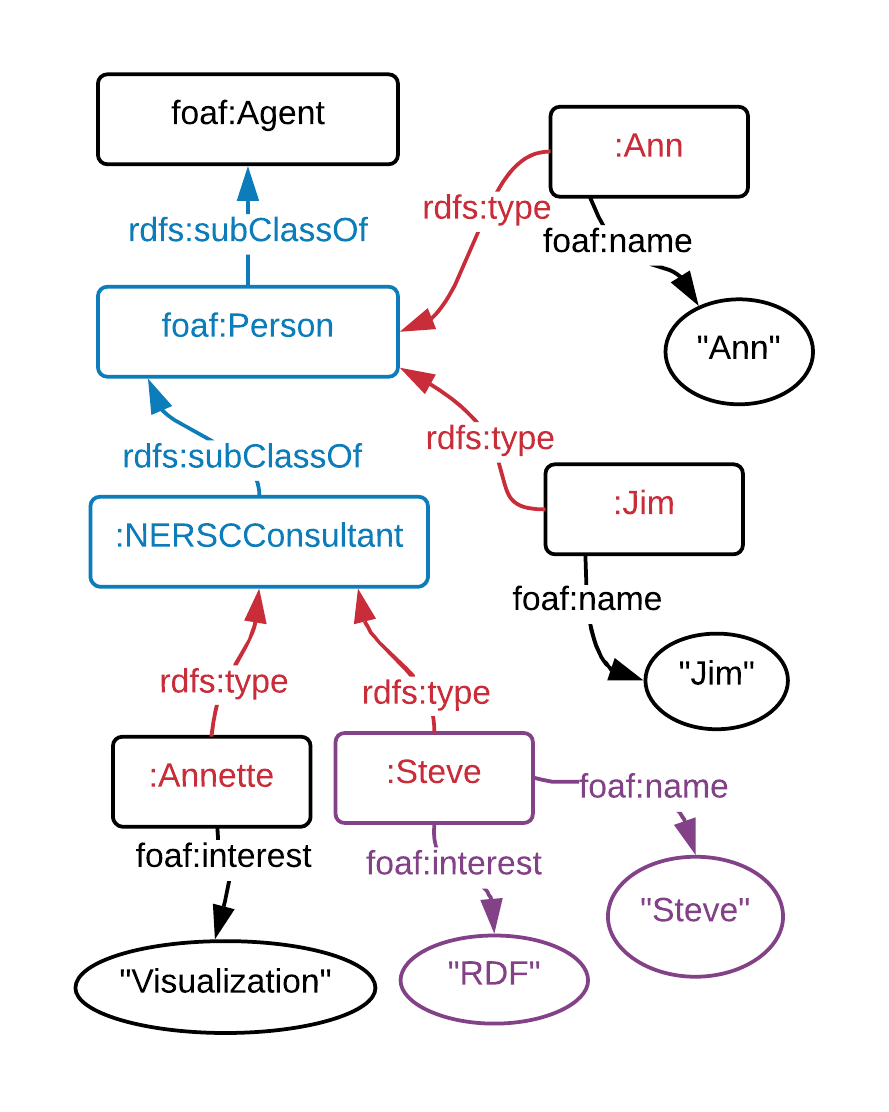
\includegraphics[width=0.4\textwidth]{sparql.png}
\caption{Illustration of the SPARQL query in Figure~\ref{f:sparql} }
\label{f:sparql-diagram}
\end{figure}

\textcolor{red}{TODO: draw this as a diagram, probably explains it better}
\textcolor{red}{TODO: prob need a ref to an "intro to semantic web" resource}

RDF provides a decentralized mechanism for publishing information in a
machine-readable and searchable way, neatly meeting our requirements
(2) and (5). Furthermore, RDF allows us to use an established ecosystem of 
tools and libraries to achieve our goals.

\subsubsection{The vocabulary}

The key classes and predicates forming our vocabulary are illustrated in 
Figure~\ref{f:logset-classes}. Figure~\ref{f:logset-classes-nodes} provides 
examples of nodes in a graph corresponding to each class, and an 
illustration of how RDF descriptions of different \texttt{LogSet}s published 
in different places form a single, global graph is show in 
Figure~\ref{f:logset-example}. Particularly, Figure~\ref{f:logset-example}
shows how the vocabulary can be used to publish data dictionaries 
describing different \texttt{SubjectType}s and \texttt{LogSeries}.

The vocabulary is extended and specialized 
from the Data Catalog Vocabulary \textcolor{red}{cite}. The meaning, 
reason and usage of each are as follows:

\begin{description}
\item[Catalog] \hfill

The \texttt{dcat:Catalog} class is used as an access point to LogSet datasets and 
to link disparate collections into a single graph. Catalogs are anticipated to be 
published at a site granularity: staff at a site would publish LogSets under
a URL that the staff member can access, linked to the global graph via a single 
entry in the site Catalog. (The mechanism for this can be as simple as a pull
request to a Github repository).

\texttt{Catalog}s can use \texttt{rdfs:seeAlso} properties to link to other 
catalogs and to data dictionary

\item[LogSet] \hfill

A collection of logs related in system and access and timespan,
for example the logs collected in a \texttt{p0-} directory in the SMW of a Cray
XC for a single boot session. The \texttt{LogSet} should provide a description
of the data and contact information and is an entry point to metadata for 
the \texttt{ConcreteLog}s.

Note that the \texttt{LogSet} itself doesn't necessarily have properties for 
temporal or subject information. We anticipate that these would be derived 
from the \texttt{ConcreteLog}s comprising the \texttt{LogSet}.

A \texttt{LogSet} might be a closed archive or might be ``open'', that is' 
acquiring new logs over time. This is indicated via the \texttt{isClosed} 
property, ..

\item[ConcreteLog] \hfill

A \texttt{ConcreteLog} describes a specific, concrete source of log entries.
This might be a log file but could also be, for example, a Slurm instance
from which job data can be obtained. 

The \texttt{accessURL} and \texttt{downloadURL} have subtly different uses,
inherited from \texttt{dcat:Distribution}. The actual data described by the 
\texttt{ConcreteLog} may not be directly accessible (due to security or 
other practical constraints), in which case an \texttt{accessURL} which 
can help a user to learn about gaining access is more suitable than a 
\texttt{downloadURL}, which is expected to provide direct access to the 
data.


The \texttt{ConcreteLog} also supports a number of properties about the
size, number of records and timespan of the data. For many data sources 
an ill-considered query might result in an excessive volume of data returned,
so these properties are intended to help users check 


\item[LogSeries] \hfill

The console log for a server is often distributed over multiple files,
and is fundamentally the same for servers of the same make at different
sites. A \texttt{LogSeries} allows the common metadata to be published
once in a common dictionary...


\item[LogFormatType]

One level more general than a \texttt{LogSeries}, a \texttt{LogFormatType}
is common to many \texttt{LogSeries}. As an example, many \texttt{LogSeries}
have the form of a \texttt{timeStampedLogFile}. Another significant 
\texttt{LogFormatType} is \texttt{sqlite3DB} (which encapsulates our 
reference implementation of the Annotation Schema~\textcolor{red}{cross-ref})

\item[Subject]
...
affects and partOf



\item[SubjectType]

Each \texttt{ConcreteLog} has a specific \texttt{Subject} - e.g. a 
\texttt{cori} or \texttt{cori\_nid00123}. It is useful to classify 
\texttt{Subject}s by their type so that for example, a researcher 
seeking HSN data can find \texttt{ConcreteLog}s about the HSN 
component of multiple clusters by querying for \texttt{ConcreteLogs}
whose \texttt{subject} is a specific \texttt{subjectType}. 

This also supports cataloging new datasets: rather than asking the
user the \texttt{subject} of each \texttt{ConcreteLog}, we can 

skos:broader, also aspectof


\end{description}

-- some key things to call out:
\begin{itemize}
\item someone publishing a logset doesn't need to know many people to get their 
      logset into the graph - a curator of their local (site) catalog is enough. 
      That curator then knows curators of at least one other catalog and thus 
      gets the local 
      subgraph into the global graph
\item someone using the graph doesn't need to know who published what - they can
      query the graph itself and get metadata about what is out there, including contact 
      information for data they don't directly have access to. This allows them to 
      solve specific access limitations in a locally-appropriate way
\end{itemize}

\begin{figure*}
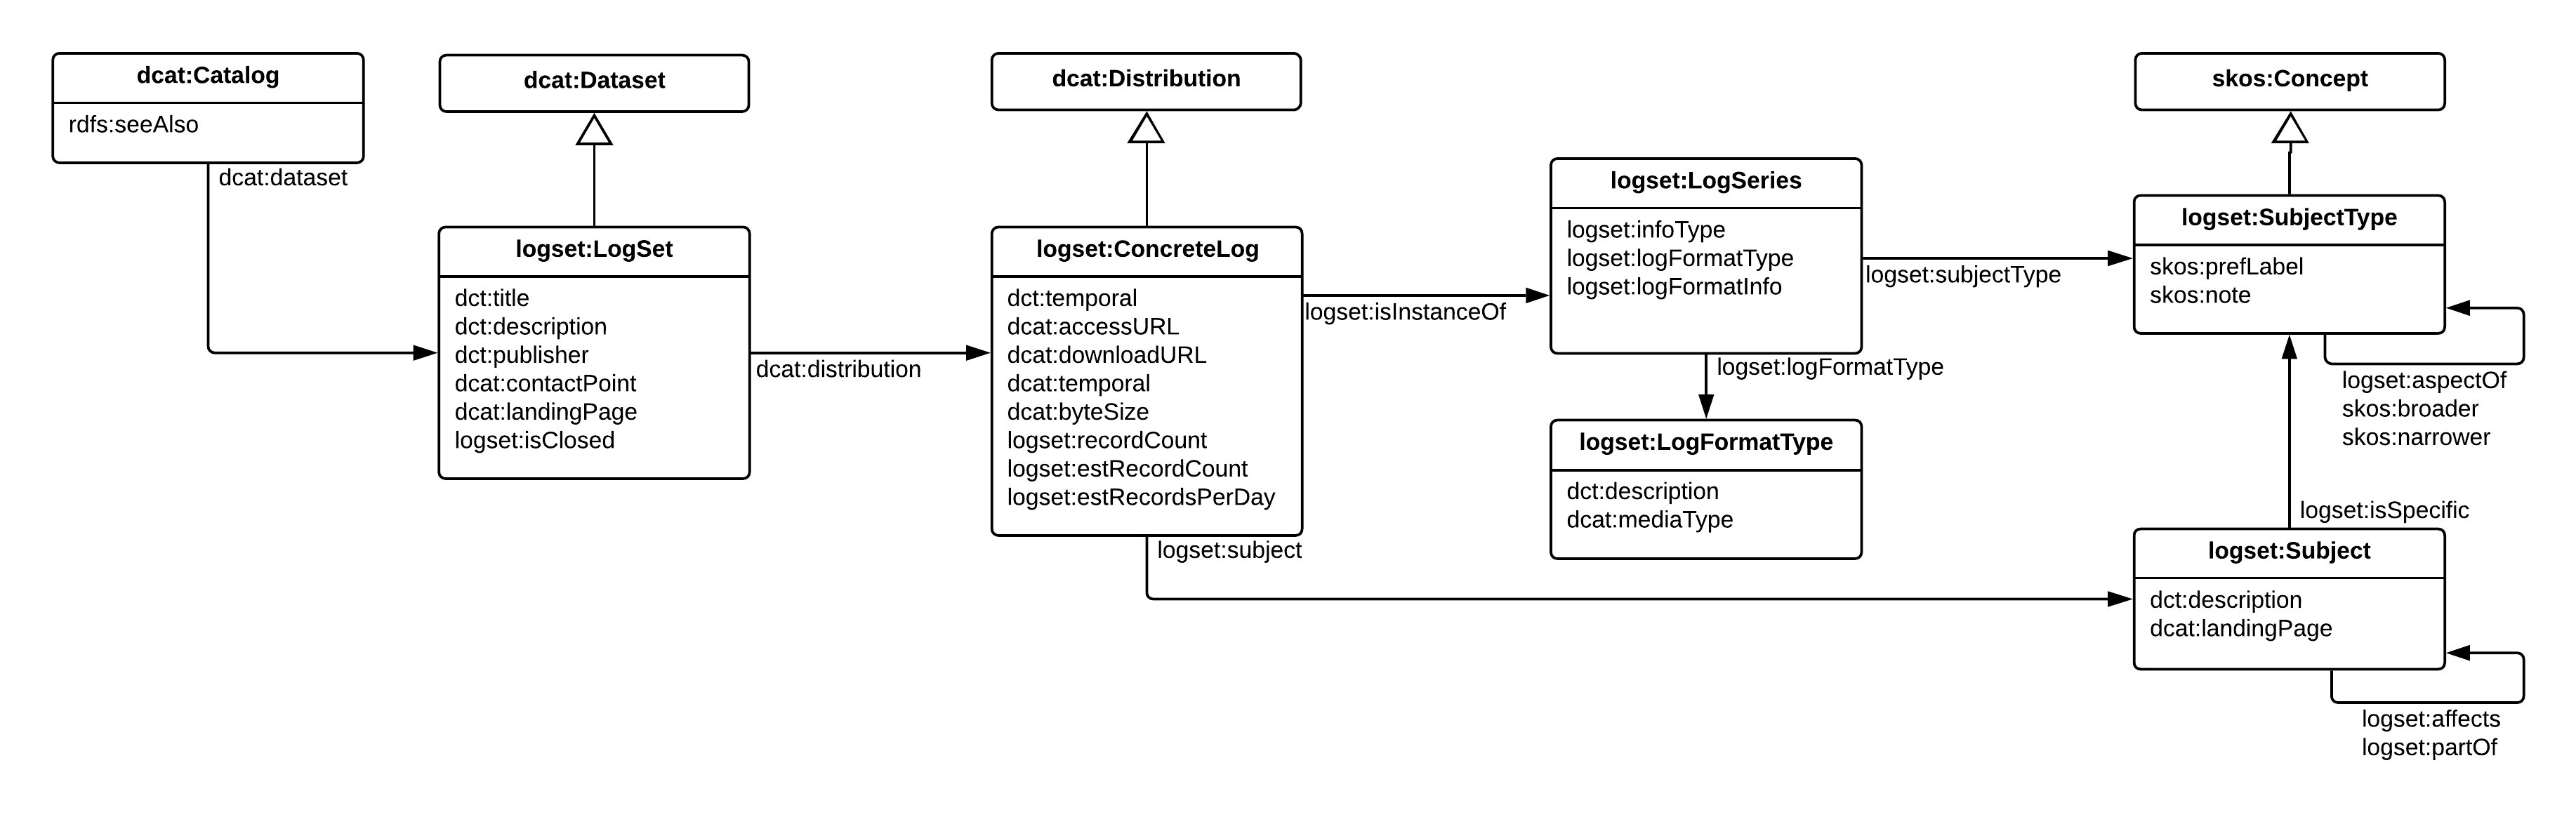
\includegraphics[width=1.0\textwidth]{logset-key-classes.png}
\caption{Key classes and predicates in the logset vocabulary. }
\label{f:logset-classes}
\end{figure*}

\begin{figure*}
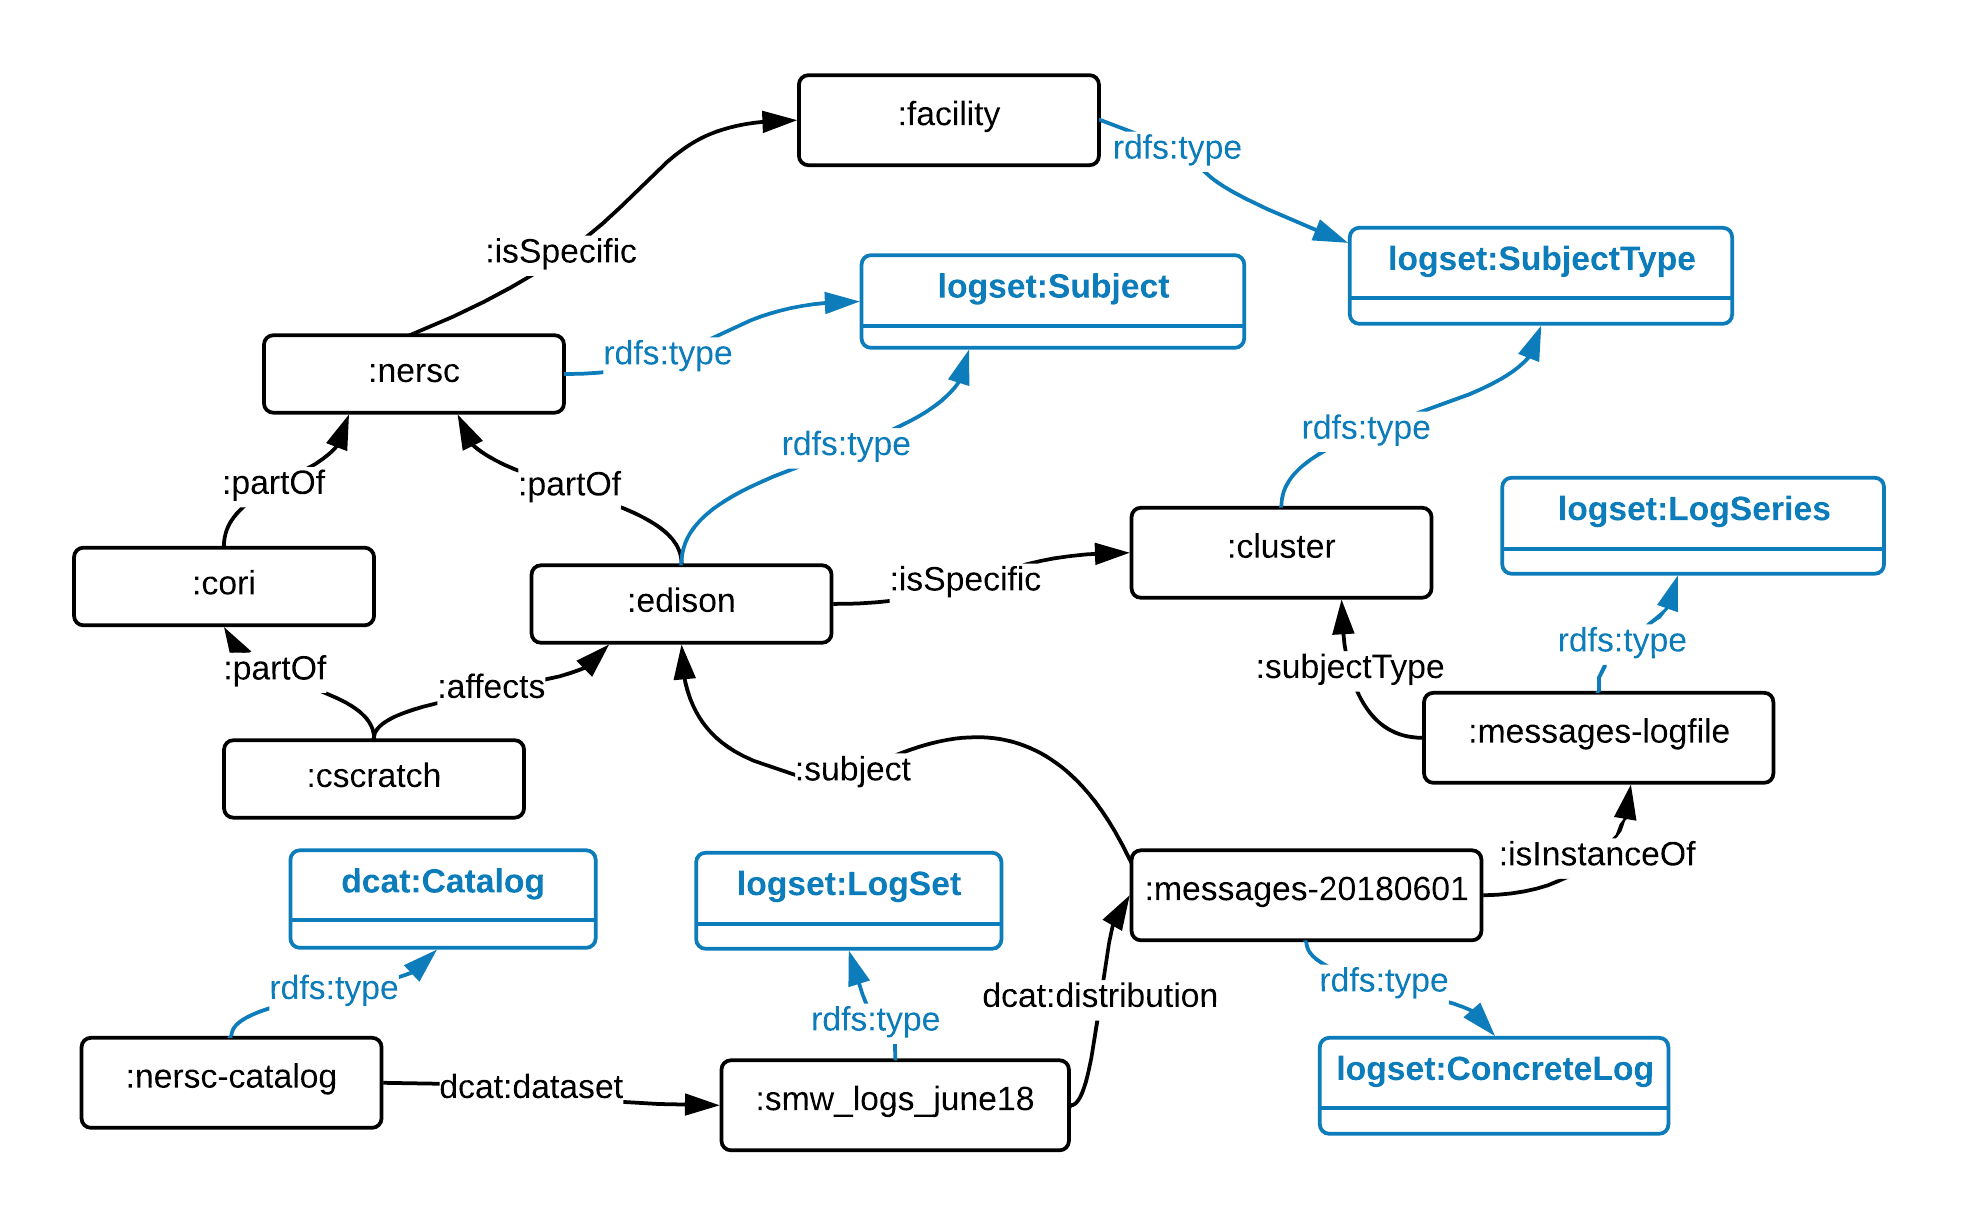
\includegraphics[width=0.9\textwidth]{logset-classes-nodes.png}
\caption{Examples of some nodes and relationships published in different places 
from different sites (indicated via color), forming a single global graph. }
\label{f:logset-classes-nodes}
\end{figure*}

\begin{figure*}
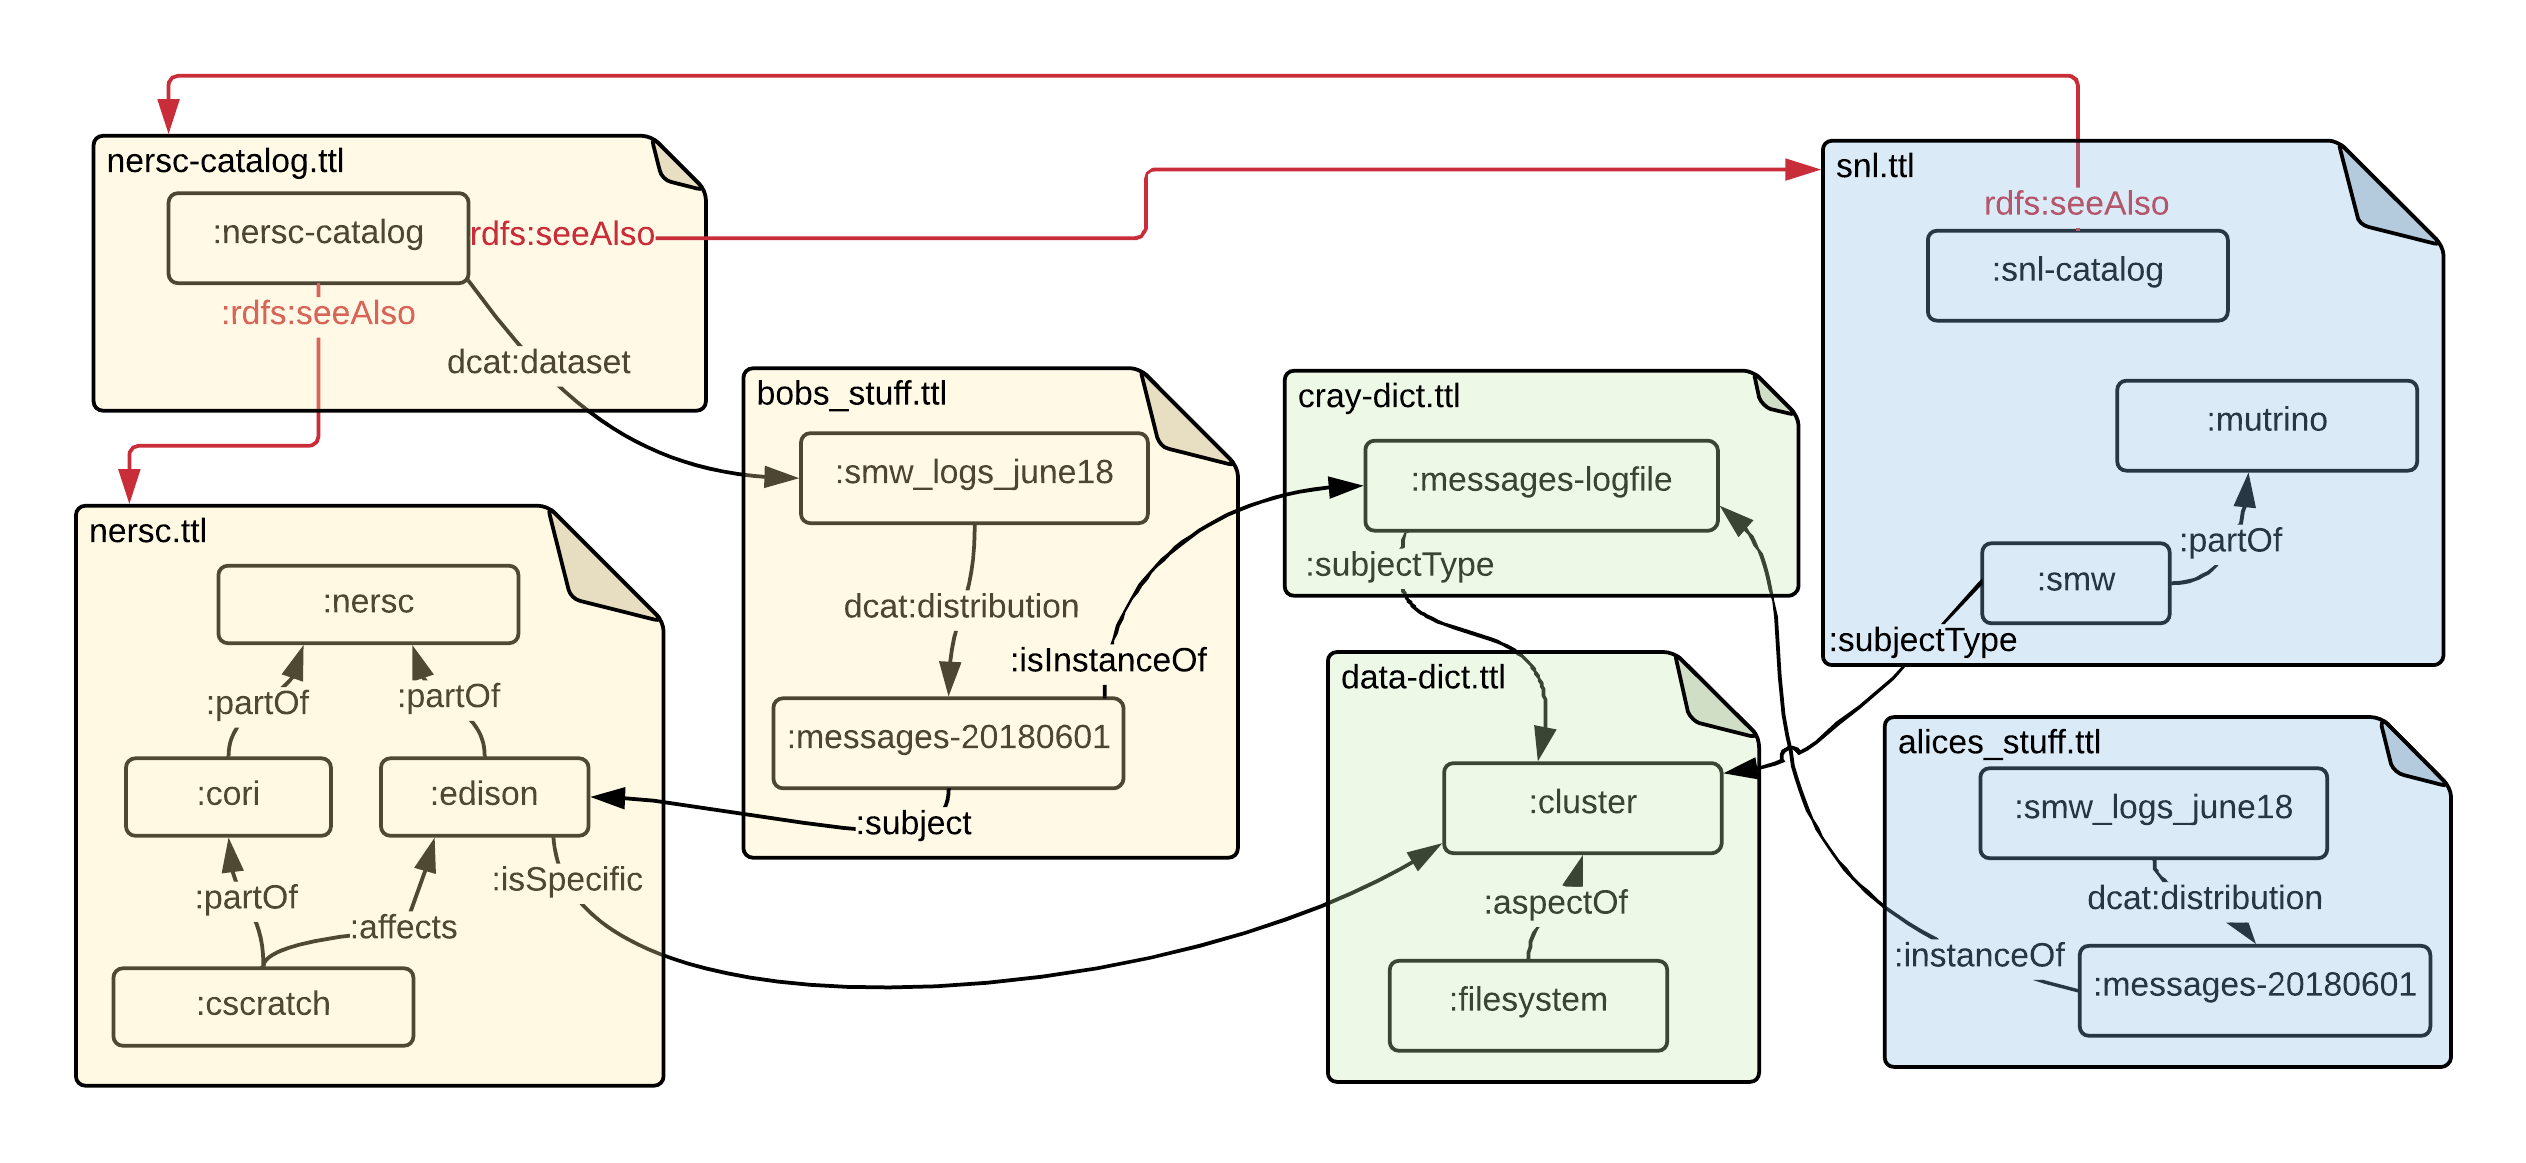
\includegraphics[width=0.9\textwidth]{logset-example.png}
\caption{Key classes and predicates in the logset vocabulary. }
\label{f:logset-example}
\end{figure*}

\subsection{Annotation Schema}

The primary goal of annotation is to provide a reduced
Some specific requirements influencing the design of our annotation schema
are:

\begin{itemize}
\item 
\item Temporal and subject (system and component) information are 
      the key fields, along with a human readable description, the 
      annotation itself.
\item The raw logfiles that the annotation concerns should be identified,
      if possible.
\item Multiple people should be able to annotate the same underlying 
      log data, and users of the annotations should be able to 
      identify annotators to request more information, if necessary.  
\item The architectural relationships between components indicated in 
      annotations should be accessible, in order to facilitate 
      traversal from an annotation of interest to annotations relating to
      components that may have impacted it.
\item Annotation fields should support searching based on the subject type 
      of an annotated event (such as a network event) or other 
      related information.
\end{itemize}



\begin{figure}
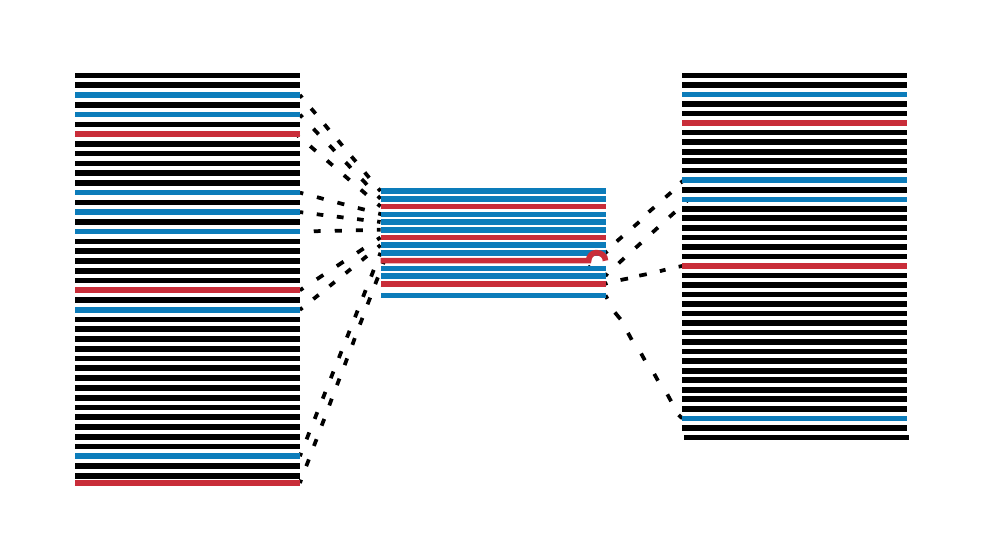
\includegraphics[width=0.4\textwidth]{annotations.png}
\caption{Annotations can collate a tractable subset of data from multiple log files into a single location.  }
\label{f:annotations}
\end{figure}

\begin{description}
\item[Catalog] \hfill

\end{description}

%In this subsection we describe the major fields necessary to support the
%architectural requirements that pertain to the annotations themselves
%(as opposed to the remote discovery infrastructure). The prototype
%implementation is an SQLite database, so we descirbe in in terms
%of that implemention, however that is not required. More generally
%this would be descirbed in terms of accessor APIs independent of
%the implementation beneath them.
The annotation schema is an SQL database definition with a central ``annotations'' table. Significant fields in the annotations table are:

The annotations table is defined as:
\begin{small}
\begin{minted}{sql}
CREATE TABLE 'annotations' (
       id             integer,
       authorid       char(3) NOT NULL,
       description    text NOT NULL,
       -- timespan of the action or event:
       starttime      datetime NOT NULL,
       endtime        datetime NOT NULL,
       -- impact of the action or event:
       startstate     text,
       endstate       text,
       systemdown     boolean,
       system         text,
       components     text,
       -- was the event manually induced?
       manual         boolean,
       -- subject type and annotation context:
       LDcatgroup     text, REFERENCES 'LDgroups'
       LDcategory     text,
       LDtag          text,
       balerpatternid integer,
       -- event source:
       logfiles       text,
       PRIMARY KEY('id','authorid')
        );
\end{minted}
\end{small}

The major fields for an annotations include \texttt{description}, \texttt{starttime}, \texttt{end time},
\texttt{system}, and \texttt{components} involved.
The description is a descriptive translation of a log messge or event (Examples
are given in Section~\ref{s:examples}); it is this description to which we
mainly refer when we refer to an annotation.
The \texttt{authorid} identifies the author of an annotation, who
is responsible for the determination of the content of the assignable fields
(such as the description); the authorid and annotation id together form a unique key.
Time and component fields refer to a specific instance of a log line or event
occurence. Thus multiple annotated log line instances may share the same description,
but have different time and component values.

Other information is used to help with context and search.
For example, \texttt{startstate} and \texttt{endstate}, which
are subjective and can be used to record things like a component
that starts a faulty but is repaired by the action of the annotations,
for example, if the event is recording that a DIMM was changed.
\texttt{Systemdown} is meant to aid in the search for events that result
in full system failure.

\texttt{Manual} is used to indicate manually performed
events, such as an administrator action to take down a node as opposed
to the system taking down a node because it failed a health check.
Knowledge of this can be used to more accurately determine the
number of true failure events and for assessing the effectiveness
and availability of system resilience mechansims vs required
human intervention.

A set of fields, \texttt{LDXXX} are available to give contextual inforatmion.
At the moment only \texttt{LDcategory} is used; this is used to define the major
subsystem relevant to the annotation. The current options are: \texttt{node/blade},
\texttt{scheduler}, \texttt{storage}, \texttt{network}, \texttt{cooling/facilities/sensors},
\texttt{power}, \texttt{system software}, \texttt{datawarp}, and \texttt{unknown}.

Note that event may have many relationships. We choose to limit them to one each to address
the requirement of searchability. It is expected that exploration will facilitate dsicovery
of events, even when the first order assocation may be off; also discovery of assocationed
events in different subsytems can help understanding of how events propagate in a system.

Annotations may also refer to other annotations; this is called a \texttt{metaannotation}.
An example might be where an annotation refers to a particular facilities
test and a meta annotations refers to the entire set of tests.

\texttt{Components} can include the compute and any supporting subsystems,
such as storage and facilities related elements. For the Cray system
itself, we define \texttt{node}, \texttt{blade}, \texttt{chassis},
\texttt{cabinet}, \texttt{router}, \texttt{tile}, \texttt{link}, \texttt{nic},
\texttt{smw}, and \texttt{other}.

In order to enable dsicovery of events which are either reported on related
compoentns or that propagate amont components we support the defintion
of \texttt{architectures}. For the Cray system itself, we define three.

The \texttt{physical} architecture consists of parent-child or
container-contained assocations, such as a cabinet is the parent of
3 chassis. For the network components, the router is a child of the blade.
he router is a parent of the links and nics. The physical architecture
can be populated from system defintation (e.g., XE or XC with the
correct number of cabinets for a system).

In order to support the fact that components may be identified by differnet
names in different log messages, an \texttt{alias} table defines those conventions.
This is largely cname, nid, and IP addresses determined from \texttt{/etc/hosts}
or the output for \texttt{rtr --system-map}.

The \texttt{router} architecture includes the network topology information
for the router (e.g., blue:black:green)
for Aries and X:Y:Z for gemini). The router information can be populated from
the system-map output or the otuput of \texttt{rtr --interconnect}.
The \texttt{link} architecture represents the network link connectivity,
consisting of type (e.g., Blue, X+) and the tile endpoints obtained
from the interconnect output.

The \texttt{link} architecuture supports determination if an event affects the
components at teh other end of a network link. The router architecutre
supports determination of proximity of events in the network topology.
We chose to separate architecutres in order to enable different
search and interpreation of events which affect components with
different \texttt{association} with each other. \texttt{associations}
include \texttt{parent-child: component-component} as opposed to
\texttt{parent-child: router tile}, or \texttt{peer: HSN link}
as opposed to \texttt{peer: Router-NIC} or \texttt{peer: NIC-Proc}.
To represent more globally associated, such as SMW
events which can directly affect all components, we define
a \texttt{supremum} relationship.

In the prototype, we define all architectures and relationships,
however we currently prinipally search the physical topology only
and support recursive search up and down, including for supremum
relationships. We are working on tools to better enable search of
the multiple architecture represenations.

In order to determine the effect of events on jobs, we also
intend that job data be made availble with the annotations.
We expect only the current common fields (e.g., starttime,
endtime, components, etc) exposed in scheulder logs or
interfaces.








\subsection{Tools}
\begin{itemize}
\item get.py for querying an annotation database
\item what do we have for building an annotation database? (Ann's tool for ingesting the mutrino and jobs info?)
\item framework for working with rdf graph

(plan is to have cataloging and running general queries supported at least, and ideally also slicing-and-fetching of timestamped logs in line-per-timestamp format)
\end{itemize}


- talk about why, eg rdf because it is machine readable, supports adding tools etc over time 


To faciliate the creation of log line annotaitons
and the identification of the occurences of events to be annotated,
we have been using two tools.

LogDiver~\cite{LogDiver} is a tool developed by UIUC which includes a set of regular expressions defining
events in log files of interest; the regular expressions are associated with categorizations
which are a subset of those described in the previous section; the
category name, \texttt{LDxxx}, was chosen to refelct our intention to map to the
Log Diver categroizations where possible.
LogDiver itself is used to discover the occurences of the regular
expresssions in the logs and to determine statistics and infroamtin about event sequences
such as statistics of failure events, or of timigns of failures and recoveries.
LogDiver, or any such regex-based tool (e.g., SEC~\cite{SEC}) can be used to efficiently extract events
and annotate them, based on the intention of the extistence of the regex.

For the dataset descirbed in this work, we prinicpally used Baler~\cite{Baler} for
identifying the log lines to be annotated and for extracing them from the dataset.
Baler extracts patterns from log files without requiring aprior knowledge of
regex. Rather, Baler takes dictionaries of ''words''; words appearing in the log lines
are the passed through to the pattern and non-words become a wildcard in the pattern.
Wildcards of certain formats, for example numbers, hex dumps, char arrays, hostnames and link names
(in cname format for Cray systems) are represented as that formatted type in the pattern.
For example, every instance of the log message \texttt{mutrino-smw 24626 found\_critical\_aries\_error: Processing ''PCI-e CMPL\_TIMEOUT'' critical error (0x660e)}
is represented by the pattern \texttt{<host> nlrd <pid> found\_critical\_aries\_error: Processing ''* *\_TIMEOUT'' critical error (<num>)}.
This illustrates where words, formatted wildcards, and unformatted wildcards (represented by \texttt{*}) appear in the pattern.

For Cray systems, we augment
the dictionary with an architecture specific dictionary of about 100 words (e.g., Lustre, DIMM).
For 3 months of data from our Trinity test system, Mutrino, a 100 node XC 40,
we had over 120 million text log lines which were reduced to 15500 patterns. To further identify patterns
of interest, we weight the patterns by the occurence of 50 weighted
keywords (e.g., congestion = 1.5, error = 1.5, degrade = 0.75). This further reduced the patterns
to 2500 significantly weighted patterns. For example the pattern
\texttt{<host> nlrd <pid> ***ERROR***: Link recovery operation failed; error <num>} has
an aggregate weight of 5.5. From those, we chose 150
patterns to annotate with enhanced descirptions. This resulted in about 860,000
annotated log line instances.

It is our intention to
build a plugin to interface with Baler, and support the annotations there,
however in the prototype, we merely annotated the extracted patterns from
Baler and loaded them into the database.
We do, however, include the Baler pattern id in the annotation fields
for reference ease; only the annotation description, not the original log line nor the pattern
are stored in the annotation database.

Some example patterns, from which the originating log line will be obvious, and
the resulting annotation used in this work, are given in Figure~\ref{f:baler}

\begin{figure*}
\begin{annol}

Baler pattern, preceeded by weight (W=#) and balerpatternid number:
(W=5)        258   HWERR[<host>][<num>]:<num>:SSID RSP A_STATUS_ORB_TIMEOUT Error:*=<num>:*=<num>:*=<num>
Annotation:
authorid:acg  description: 'ORB timeout waiting on outstanding request(s) in the buffer'  LDcatgroup: NE

Baler pattern and weight:
(W=3.75)     498   <host> nlrd <pid> do_set_alerts: <num> links failed, <num> blades failed, <num> blade critical faults, *_in_progress <num>, *_*_reroute <num>; reroute required
Annotation:
authorid:acg  description: 'Setting alerts due to failures. A network reroute is required' LDcatgroup: NE

Baler pattern and weight:
(W=3.25)     748   <host> nlrd <pid> ***ERROR***: Warm swap operation failed; error <num>
Annotation:
authorid:acg description: 'Warm swap failed. This is in response to a operation intended to reset/reinit/replace a component (including network components).' LDcatgroup: NO

Baler pattern and weight:
(W=1.5)      705   <host> nlrd <pid> responder_work_*: Top <num> nodes involved with network congestion
Annotation:
authorid:acg description 'System computing and listing congestion candidate applications' LDcatgroup:NE
\end{annol}
\caption{Example Baler patterns extracted from log lines and their annotated versions. Events to annotate are based on
knowledge of significant events. Annotation descriptions can provide additional context to non-self-explanatory log messages.}
\label{f:baler}
\end{figure*}

\begin{figure*}
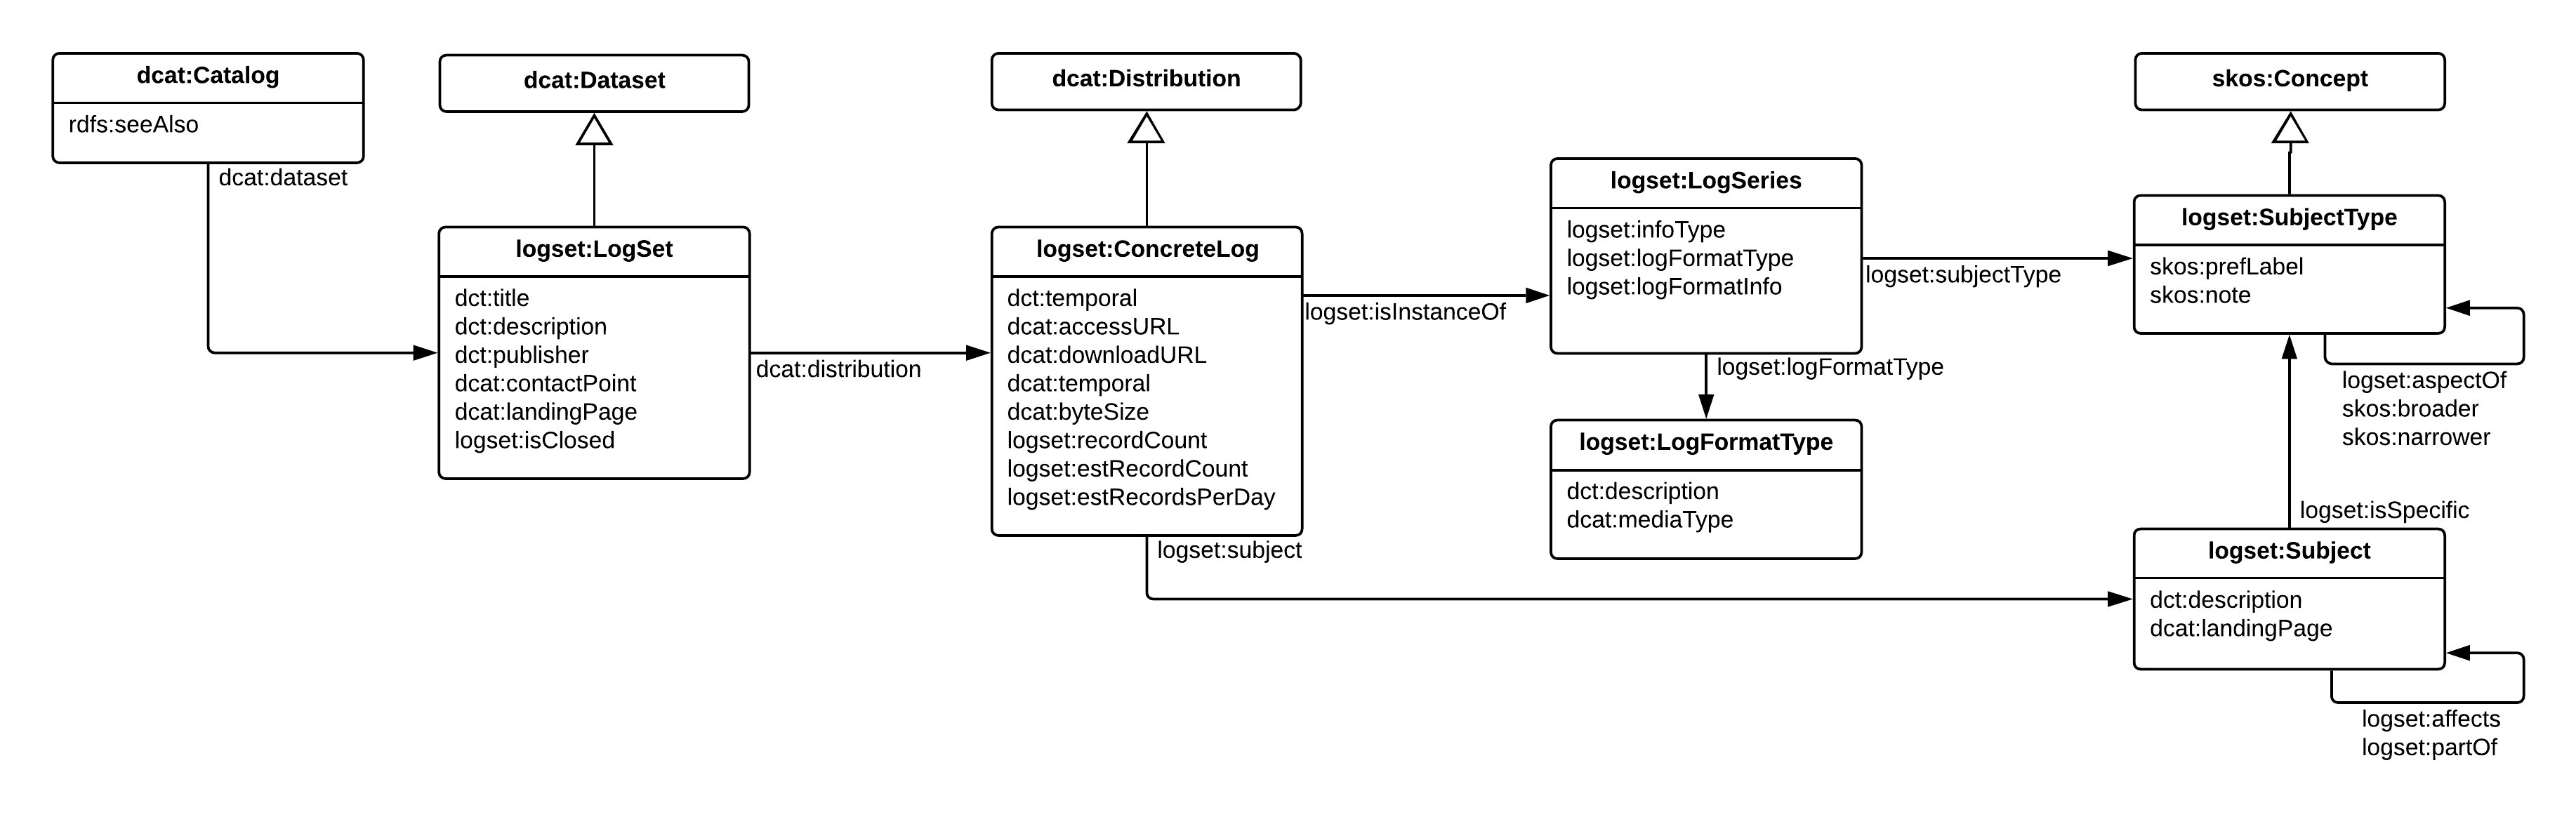
\includegraphics[width=0.9\textwidth]{logset-key-classes.png}
\caption{logset key classes}
\end{figure*}













